\section{Introduction}
		\hspace{10mm}Blockchain technology has been a disruptive force in this world. Originally, that disruption was felt in the financial sector with Bitcoin. This relegation to the financial sector existed because the Bitcoin scripting language Script was intentionally non-Turing complete; perfect for its Use Case as a cryptocurrency, but otherwise significantly under-powered for general applications. However, it wasn't long until the next level came in the form of Ethereum which introduced a Turing-complete scripting language along side its cryptocurrency offering. This opened up the world to the possibility of decentralized applications (dApps). While those platforms were necessarily public and open, others still thought about other Use Cases that would benefit from the use of this type of distributed technology -- ledgers in the form of cryptographically connected blocks, decentralized node consensus, scripting to build applications on these platforms, etc. -- in a private and permissioned space. One of those offerings was a system, itself defined and built by a consortium of organizations (from Intel to IBM), maintained by The Linux Foundation called The Hyperledger Project.\\
	
		\hspace{10mm}FabSec (short for Fabric Security) is an exploration in the potential of using Hyperledger Fabric's Distributed Ledger Technology\footnote{A note about terminology: You'll see a few terms being used here such as Consortium Blockchain and Distributed Ledger. For the purposes of this project, as well as many others these are interchangeable. This interchangeability holds because a Blockchain system at its base is nothing more than a Distributed Ledger of transactions. Another example of this seen later is Chaincode vs Smart Contracts -- similar terms that can be used interchangeably.} as a dedicated overlay security network. Hyperledger is an ecosystem of different tools, libraries and frameworks for creating different types of Blockchains: from private and permissioned to public and permissionless. Fabric is one of those Blockchain frameworks. It allows multiple actors to share a blockchain between themselves for any Use Case to which they could think to apply it. I will go into Fabric more in depth in its own section coming up, but first let's dive into some of the background concepts.\\
		
	\subsection{Conceptual Background}
		\hspace{10mm}To get the reader up to speed, let's looks are some of the terms used above: What is Computer Security? What is the Blockchain, and where did it come from? How did the blockchain evolve into a system used outside of financial sector? And what does that mean moving forward?
		
		\subsubsection{Computer Security}
			\hspace{10mm}Computer Security\footnote{Again on the terminology front, Computer Security as I am using it can involve both online and offline security. Sometimes a distinction is made of Cyber or Web Security for online and Computer or Binary Security for offline. There are also deeper lines drawn like Information Security, Mobile Security, Application Security, etc. For the purposes of this section, there is no distinction between these terms.} is a broad topic, and, as with most of these background concepts, you can have full papers dedicated to this topic. Broadly, however, you have two sides to Computer Security: offensive and defensive. This project will cover the defensive side. The Defensive Side concerns itself with topics such as how do I maintain a system in which users, resources, and data can be protected, safe, and available? This is often encapsulated in the notion of the CIA (Confidentiality, Integrity, and Availability) Triad.\\
			
		\subsubsection{Bitcoin and Blockchain}
			\hspace{10mm}Bitcoin is a decentralized financial system created by Shatoshi Nakamoto\footnote{Shatoshi Nakamoto is a pseudonym, however, and the real person behind Bitcoin's invention is rather unknown}. It was created with the idea that there should be a decentralized financial system unlike the US Dollar or EU Euro. One that was kept out of the control of the state and, by extension, out of control of centralized banks. The Bitcoin System consists of untrusting nodes on a network which maintain their own copy of a shared ledger of transactions. Specifically, this ledger keeps track of the Unspent Transaction Outputs, or UTXOs, of all the transactions between two or more parties that will consume old UTXOs and create new UTXOs. The sum of values that a certain set of UTXOs, say that belong to an individual, adds up to is that amount of Bitcoin that individual has. To make sure that these values on the ledger weren't modified by nefarious actors -- after all, each untrusted node on the network has a copy of this running ledger -- a special Data Structure called the Blockchain was created.\\
			
		\begin{figure}[h!]
		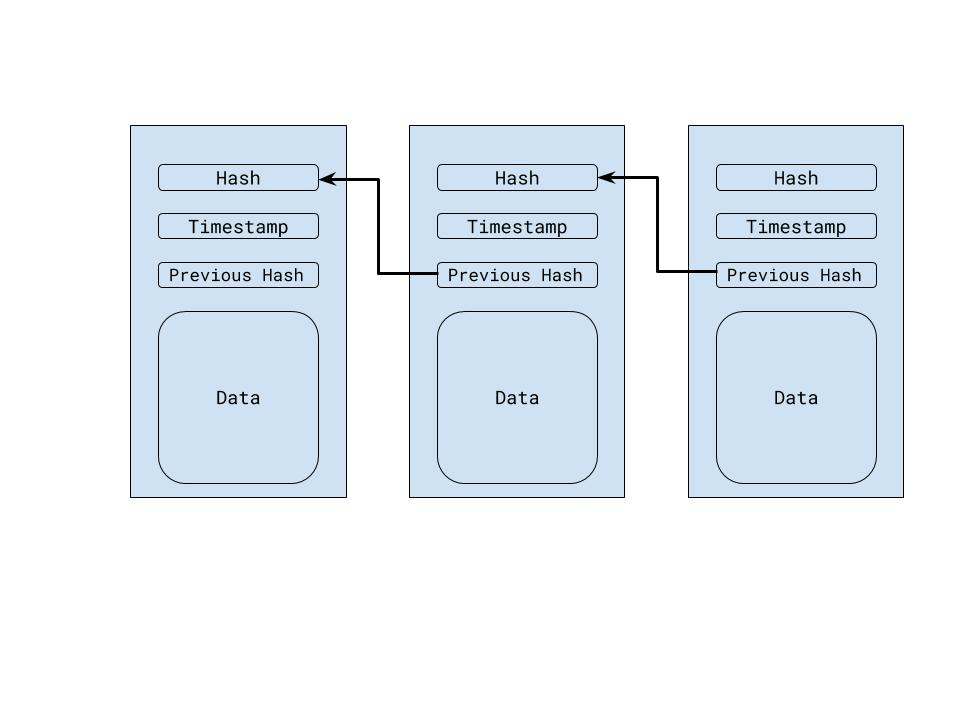
\includegraphics[width=\textwidth]{./fabsec-report-introduction/blockchain-diagram.jpg}
		\caption{A Simplified View of the Blockchain}
		\end{figure}
		
			\hspace{10mm}The idea of the Blockchain can be broken down into its two constituent words: Block and Chain. A Block is a grouping of these transactions as trusted, verified, and accepted by special nodes called Miners\footnote{This paper won't go into detail of what those Miners do exactly. Just know that they are a crucial part of how the Bitcoin system can be trustworthy in an untrusted environment.} with some Metadata added. The two important parts of this metadata are the Hash belonging to the block which is all of the block's contents run through a hashing algorithm and the hash of the previous block in the chain. The previous hash is part of the the information that gets hashed for any new blocks being added. This has the consequence of having all these block "chained" together through the hashing of previous material. This holds since if one bit of information is changed anywhere in the chain, the hashing avalanche effect states that all of the previous hashes will be fundamentally and drastically different. This allows for checksumming. That is, checking that a newly formed hash is the same as a given, usually trusted, hash. So, here we have all of these "Blocks" that a "Chained" together via the mathematics of Hashing.\\
			
		\subsubsection{Ethereum and Smart Contracts}
			\hspace{10mm}As mentioned before, Bitcoin also has a scripting language called Script. The details of what Script does is not particularly relevant to this paper other than it was a way for Bitcoin to be automated, specifically checking if the aforementioned hashes were correct. This scripting was completely, and intentionally, under-powered. It didn't have loops, and it had limited conditional logic -- as well as other missing components that would deem it not Turing-complete. This was so, again, nefarious actors couldn't break the system such as creating infinite loops. However, one person saw a lot of promise in this idea of not only a shared ledger but also that of shared processes via scripting: Vitalik Buterin. Vitalik created a new Cryptocurrency offering called Ethereum. Like Bitcoin, it had a blockchain of financial transaction associated with it, however unlike Bitcoin it had a fully featured Turing-complete scripting language associated with it which allowed for the formation of Smart Contracts.\\
			\hspace{10mm}Smart Contracts allowed users to create very intricate distributed programs governing how Ether -- the "coin" of Ethereum -- could be used. All of the nodes in the Ethereum network would run these scripts and verify the results and perform the resulting actions. Typically this would transfer an amount of Ether when certain conditions were met. To avoid the pitfalls of things like infinite loops, the act of running a Contract takes, itself, a small about of Ether called Gas. So, any actor creating a malicious Contract like that would run out of gas before their loop, or whatever the malicious case may be, would break the system. Developers eventually discovered that they could have things like a web-based front-end which allowed other users to connect to their contracts and use them via a web browser. With this, this idea of Decentralized Applications (dApps) were hoisted to the frontlines of the Crypto world. 
			
		\subsubsection{Decentralized Applications (dApps)}
			\hspace{10mm}Decentralized Applications are the general term for these distributed programs. They have been around since before the time of cryptocurrencies but have seen a spike in popularity now that there are these widespread dedicated networks to host them. However, at the time of writing this, they are still attempting to gain traction in a meaningful way. Still, there are a fair amount of games, betting pools, and plenty of Decentralized Finance (DiFi) applications in the dApp ecosystem. The main takeaway here for this paper is the idea of shared, or distributed, processes that take place on every node on the network to affect the shared ledger between them. This is exactly what Hyperledger Fabric's main draw is.
	
	\subsection{Project Motivation}
		\hspace{10mm}This project attempts to explore use of this technology in the security space, namely having a dedicated security network between actors. These actors can be two (or more) organizations looking to join forces and pool security resources. In fact, how this idea got started was thinking about having a dedicated security network as an overlay to something like a Wide-Area Network (WAN) specifically that of a Metropolitan-Area Network (MAN). You could have multiple organizations within a city each helping to strengthen the security mission of their networks without having that security centralized as a city is often its own ecosystem of businesses, departments, and other stakeholders. An extended hope is that this could one day be applied to non-permissioned and/or possibly public blockchains in future work.\\
	
		\hspace{10mm}The choice to start with using Fabric for this idea was the ability to have full control of the blockchain in question while the structure was being planned out and the scripts and chaincode were being developed. A public blockchain such as Etheruem sounded like too many unknown variables right out-of-the-gate. That being said, and as mentioned above, it is a hope that once the plans are solidified translating this work to a public blockchain won't be too difficult. However, something thought about after this choice was made was doubling down on the idea of using a permissioned blockchain such as Fabric for a real implementation, such as for a MAN. The beauty of the idea is that its easily translatable to many different platforms, and the group of stakeholders that create the quote-unquote "owner" of the MAN can take advantage of the different components of a Fabric network while maintain their organization agency over it, but still have the shared resources.\\
		
		For security network applications, I believe this could have great value in the realms of Public Key Infrastructure (PKI), Two-Factor Authentication (2FA), Distributed Denial of Service (DDoS) prevention, Domain Name System Security (DNSSec), and beyond! The Proof-of-Concept of this research project will be a single blockchain -- or Channel in Hyperledger parlance -- to be used as a Distributed Log Aggregator. As anyone in blue team security can tell you, the logs are everything!\\
	
	\subsection{Project Objectives}
		\hspace{10mm}The objectives of this project are:
		\begin{itemize}
			\item To demystify the Hyperledger Fabric Distributed Ledger Technology
			\item To test the applications of a permissioned blockchain system in the realm of Computer Security
			\item To explore distributed computing in a meaningful manner
		\end{itemize}
		
	\subsection{Key Achievements} 
		\hspace{10mm}This is the creator's hope that this project will find use in Distributed Ledger Technology within the domain of computer security scalability on large area networks. It is a secondary hope that this inspires more research into the topic as well.\\